As an interesting application of the code, we have investigated how $\gamma$-rays are produced in a quasi-elastic $(p,2p)$-event between $~^{17}\mathrm{N}$ and a proton target propagate through parts of the \emph{S393} experimental setup in Cave C at GSI. The $~^{17}\mathrm{N}$ nucleus had a kinetic energy of $\unit[419]{MeV/A} = \unit[7123]{MeV}$.

In order to compare \codename{} with the experimental data, its output was propagated through the experimental setup described in \autoref{tab:setup} by the Monte-Carlo \prgname{Geant4} -- used through \prgname{ggland}.
Furthermore, in order to account for the fact that photons Compton-scatter in the Crystal ball detector, energy deposits in nearby crystals are summed up according to an \emph{addback routine}. 

An addback routine is a heuristic method intended to compensate for the fact that $\gamma$-rays do not necessarily deposit all of their energy in one crystal. There are several ways to address this\footnote{see for example Simon 2013\cite{simon:2013:thesis} for an evaluation of a few different methods}, but since we are interested in comparing our simulations with experimental data, we will use this algorithm:
\begin{itemize}
\item Remove energy depositions over $\unit[10]{MeV}$ (they are too large to likely be photons)
\item Take the highest of the remaining energy depositions.
\item Add to this energy the energy deposited in neighbouring crystals at most $\unit[30]{ns}$ before or after the primary deposit, and remove these deposits afterwards. The resulting energy is taken as the total energy the $\gamma$-ray deposited in the Crystal Ball.
\item Repeat until all energy deposits are exhausted.
\end{itemize}
In addition, it was required that the energy deposited be greater than $\unit[0.1]{MeV}$: the real detector will have some threshold energy, and a lot of low energy electrons are produced in the simulations, so it is both practical and realistic to impose such a limit. The value used is somewhat arbitrary, but is low in relation to typical values.

\begin{table}
\caption{\label{tab:setup} The simulated experimental setup, with detectors, the positions of their center, and the string used to place them in \prgname{ggland}. The axes are oriented so as to produce a right-handed coordinate-system with $z$ in the beam direction, and $y$ pointing upwards. Rotations refer to rotations around these axes with respect to the origin. The Crystal Ball covers the area around the reaction, which is located at the origin in between the thin silicone strip detectors (SST 3--6).}
\begin{tabular}{l|l|r}
Detector name & Position & \prgname{ggland}-string\\\hline\hline
SST-1 & $z=\unit[11]{cm}$ & \texttt{--sst-1=z0=11cm} \\
SST-2 & $z=\unit[14]{cm}$ & \texttt{--sst-2=z0=14cm} \\
SST-3 & $y=\unit[2.05]{cm}$ & \texttt{--sst-3=z0=2.05cm,roty=90deg} \\
SST-4 & $y=\unit[-2.05]{cm}$ & \texttt{--sst-4=z0=-2.05cm,roty=90deg} \\
SST-5 & $x=\unit[2.05]{cm}$ & \texttt{--sst-5=z0=2.05cm,roty=90deg,rotz=90deg} \\
SST-6 & $x=\unit[-2.05]{cm}$ & \texttt{--sst-6=z0=-2.05cm,roty=90deg,rotz=90deg} \\
Crystal Ball & At the origin & \texttt{ --xb=z0=0cm}
\end{tabular}
\end{table}

This algorith was applied to the output of several \prgname{Geant4} simulations for different initial excitation energies. The resulting $E_\gamma$ energies, togehther with the actual gamma energies, are plotted in \autoref{fig:gamma1}. We note that the identified gamma spectrum does not change notably with the excitation energy in this range, while the actual gamma spectrum contains a larger number of outliers for higher excitation energies.

\begin{figure}
\begin{center}
\begin{tabular}{cc}
\subfloat[The identified $\gamma$ energy.]{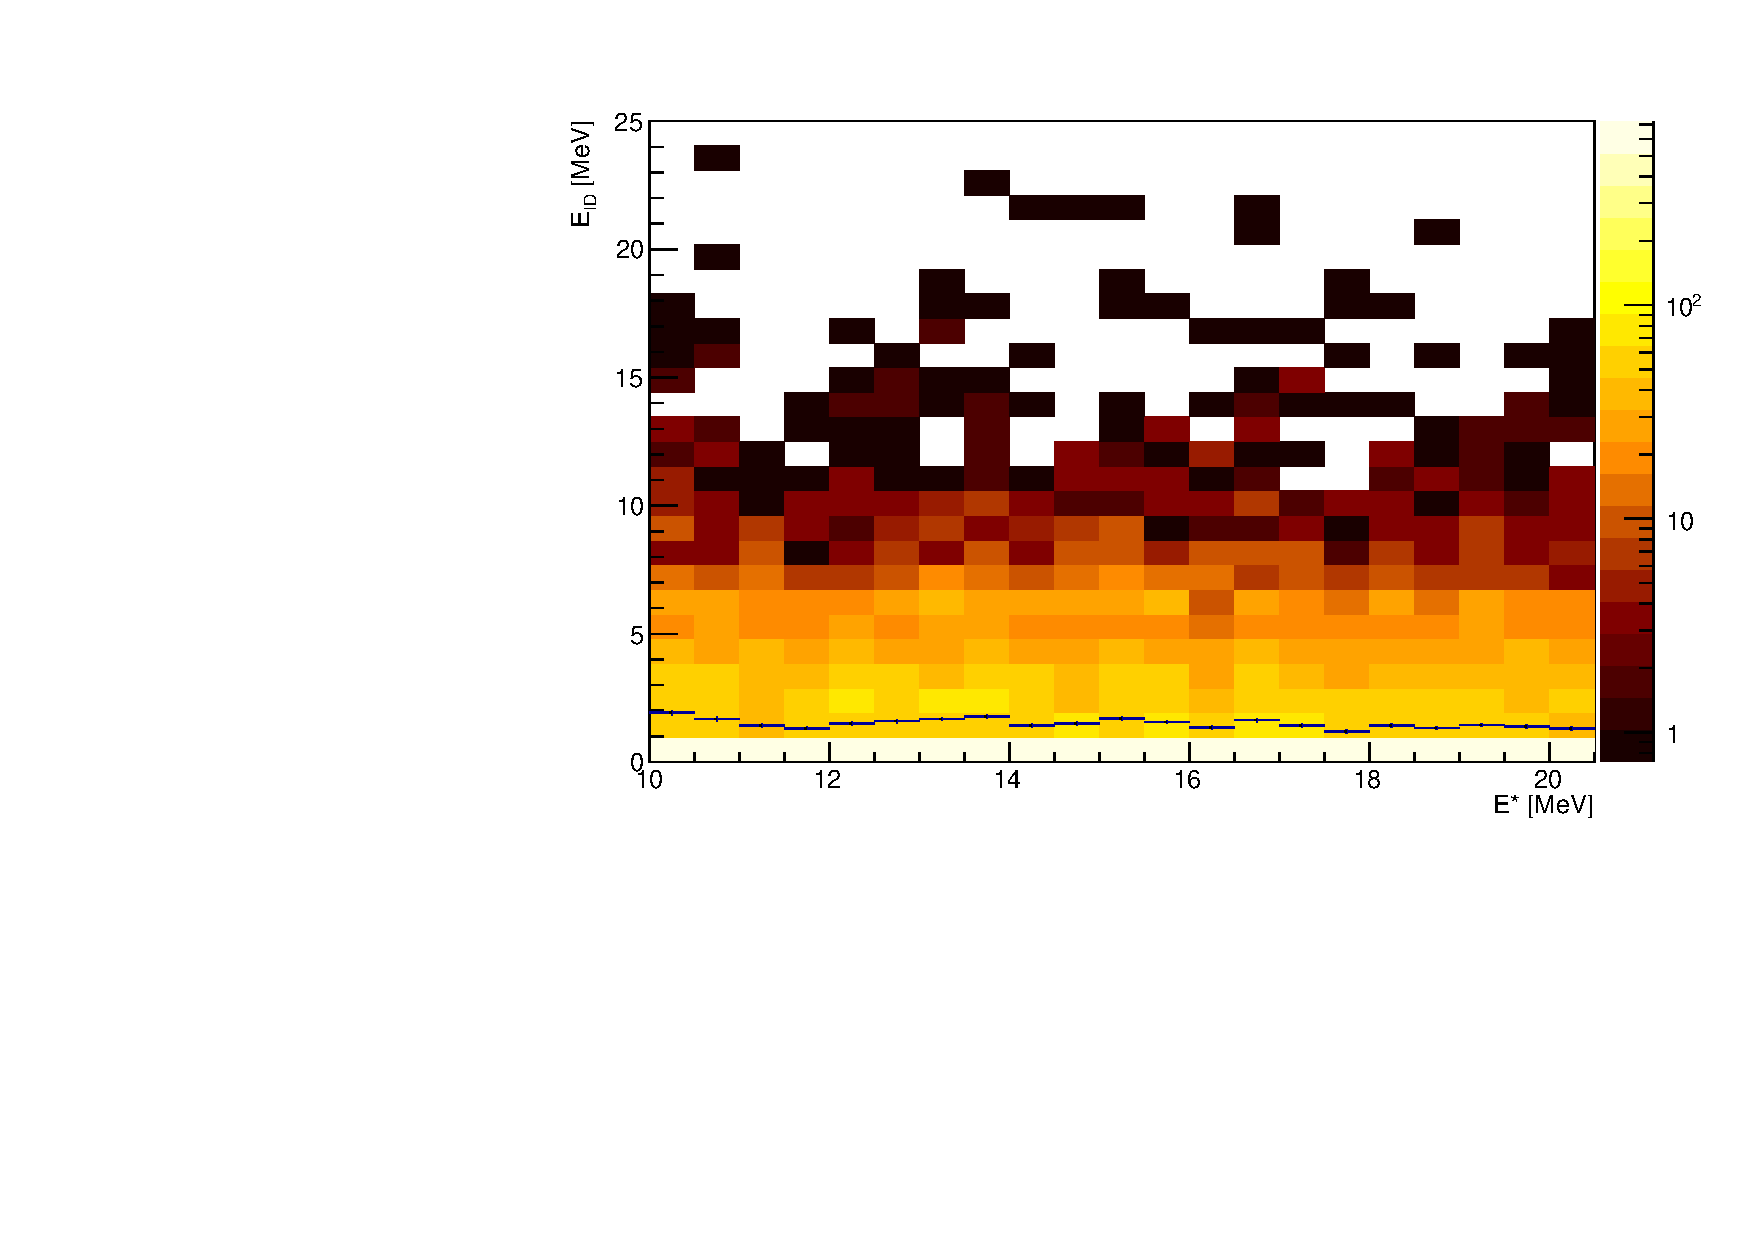
\includegraphics[width=\bredd\textwidth]{figures/gamma-mult/Eex-Eaddback.pdf}} &
\subfloat[The actual energy the $\gamma$-rays were produced with.]{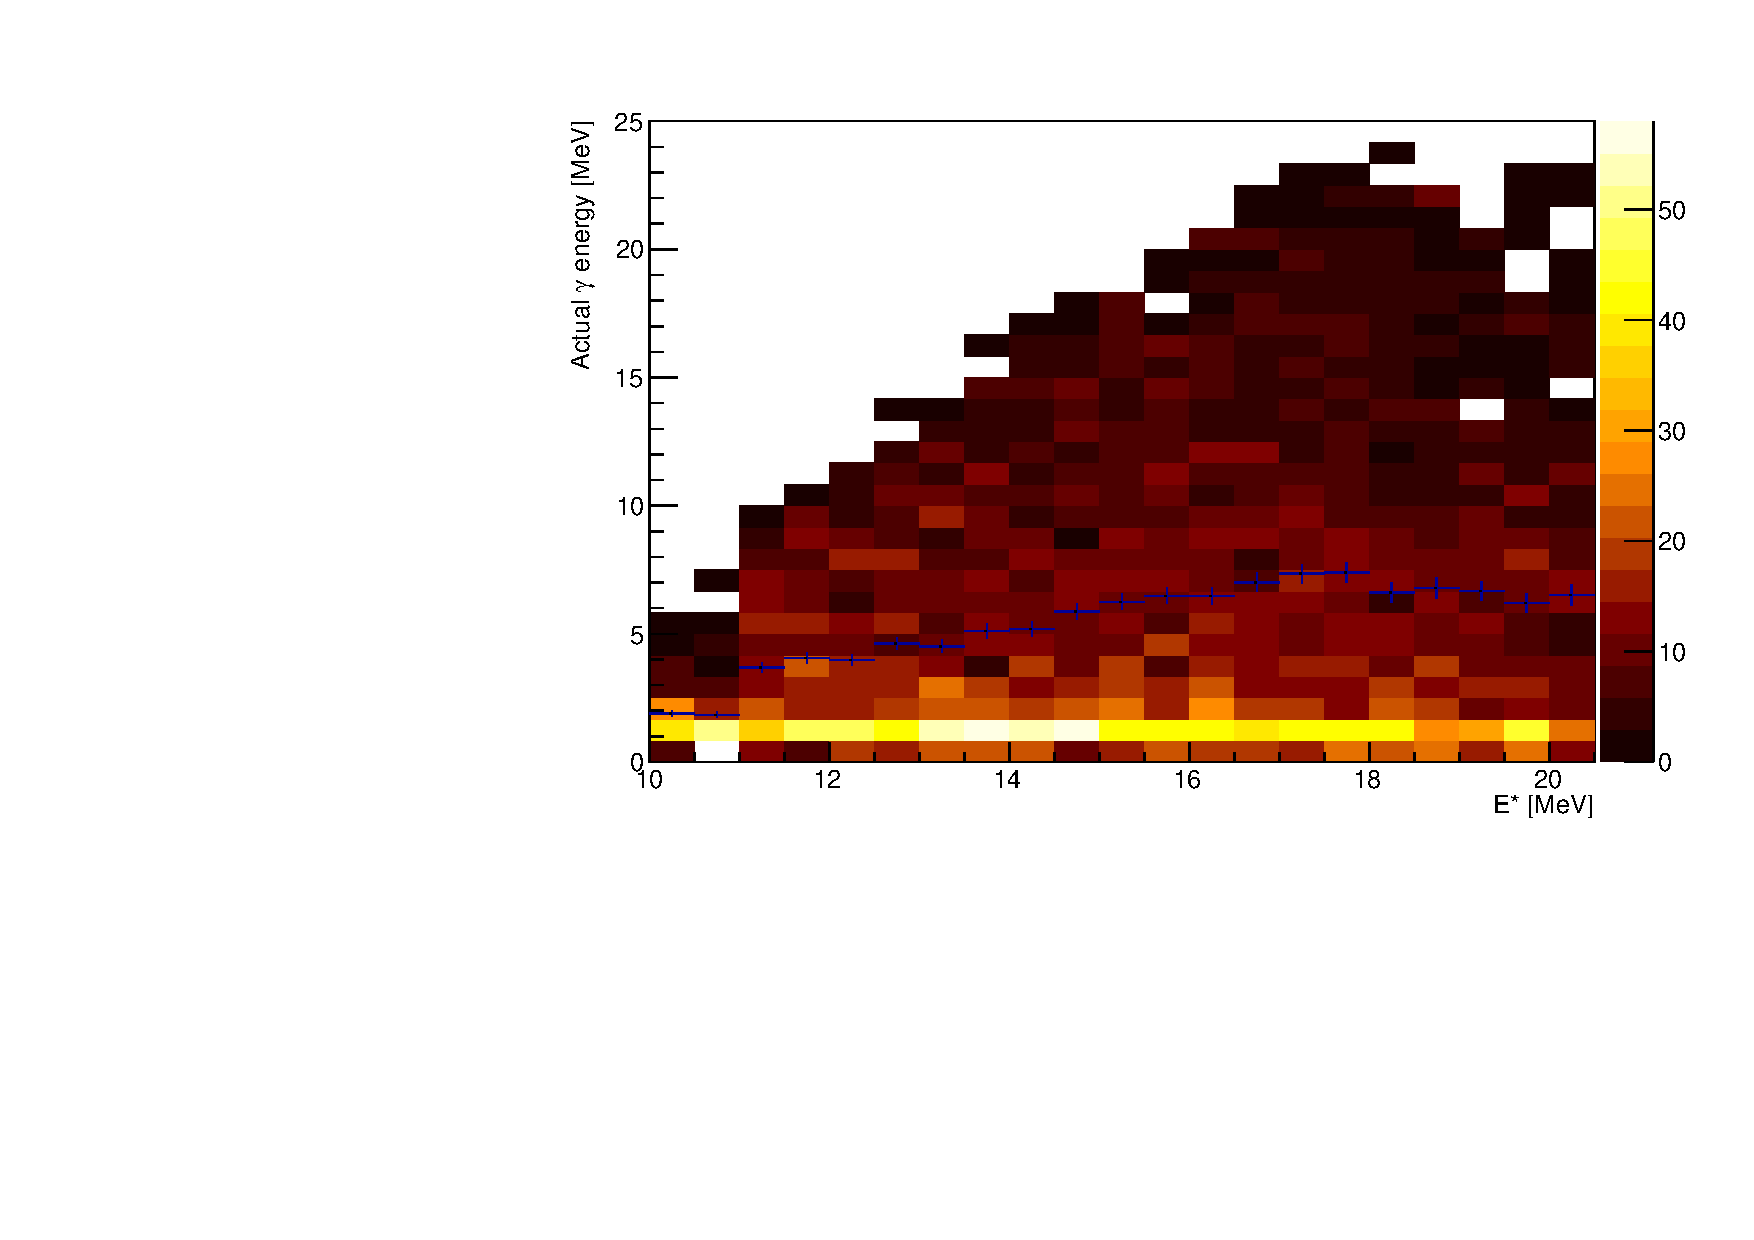
\includegraphics[width=\bredd\textwidth]{figures/gamma-mult/Eex-Eg.pdf}}
\end{tabular}
\caption{\label{fig:gamma1} The gamma-multiplicities from simulations with $~^{17}\mathrm{N}$ at a kinetic energy $T=\unit[7123]{MeV}$ undergoing a quasi-elastic $(p,2p)$ reaction with a proton at rest in the origin. The simulations were performed for prefragment excitation energies $E*$ in the interval $[10,20]\,\unit{MeV}$ with a $\unit[0.5]{MeV}$ spacing. The y-axis shows the gamma energy deposits -- event by event -- as determined by the addback routine and the actual gamma energy, respectively.}
\end{center}
\end{figure}


That being said, what is emitted by the excited nucleus and what reaches the detectors are two different things. Neither of the figures in \autoref{fig:gamma1} necessarilly tell us how much energy $\gamma$-rays actually deposited in the Crystal Ball. 
%The nucleons emitted by a more highly excited prefragment will also interact with the detectors, and could produce additional particles, as well as deposit energy in the Crystal Ball themselves.

Finally, as a test of the addback routines ability to reconstruct the number of $\gamma$-rays emitted in an event, we have in \autoref{fig:gamma2} the number of times $\gamma$-rays were identified, and the number of times they were actually generated in the reaction. Again, we see that what is identified has little to do with what is emitted in the actual simulated reaction.

That being said, it is not obvious that the number of photons \codename{} emits is entirely realistic, since the discreteness of the level density should be apparent at the energies where $\gamma$-rays are preferentially emitted. There were also a high number of low energy deposits attributed to electrons in the simulation. These so-called \emph{$\delta$ electrons} are secondary radiation produced as a result of charged particles ionizing the medium they pass through, and they could largely be filtered by imposing another, higher, threshold energy. 

\begin{figure}
\begin{center}
\begin{tabular}{cc}
\subfloat[The number of identified $\gamma$.]{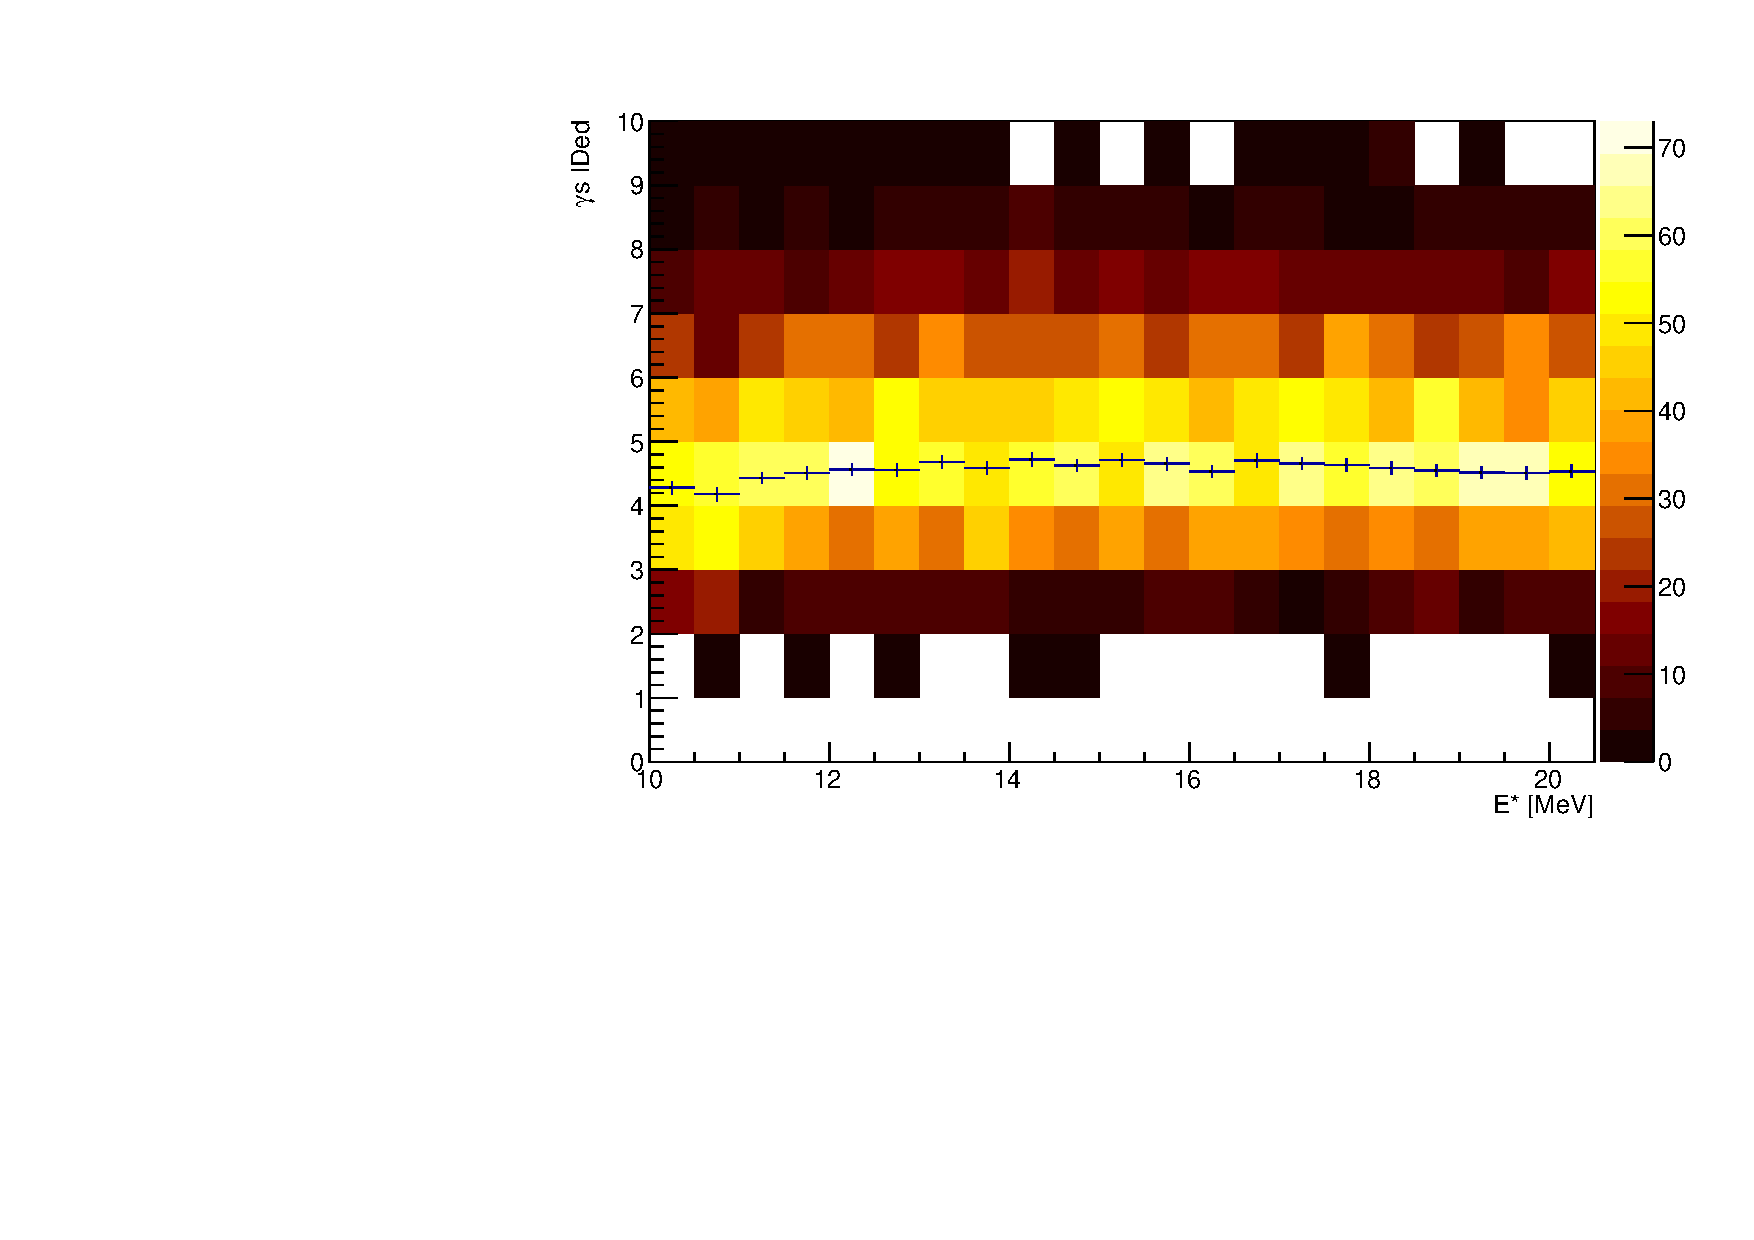
\includegraphics[width=\bredd\textwidth]{figures/gamma-mult/Ex-ig.pdf}} &
\subfloat[The actual number of $\gamma$-rays produced in the reaction between taret and projectile.]{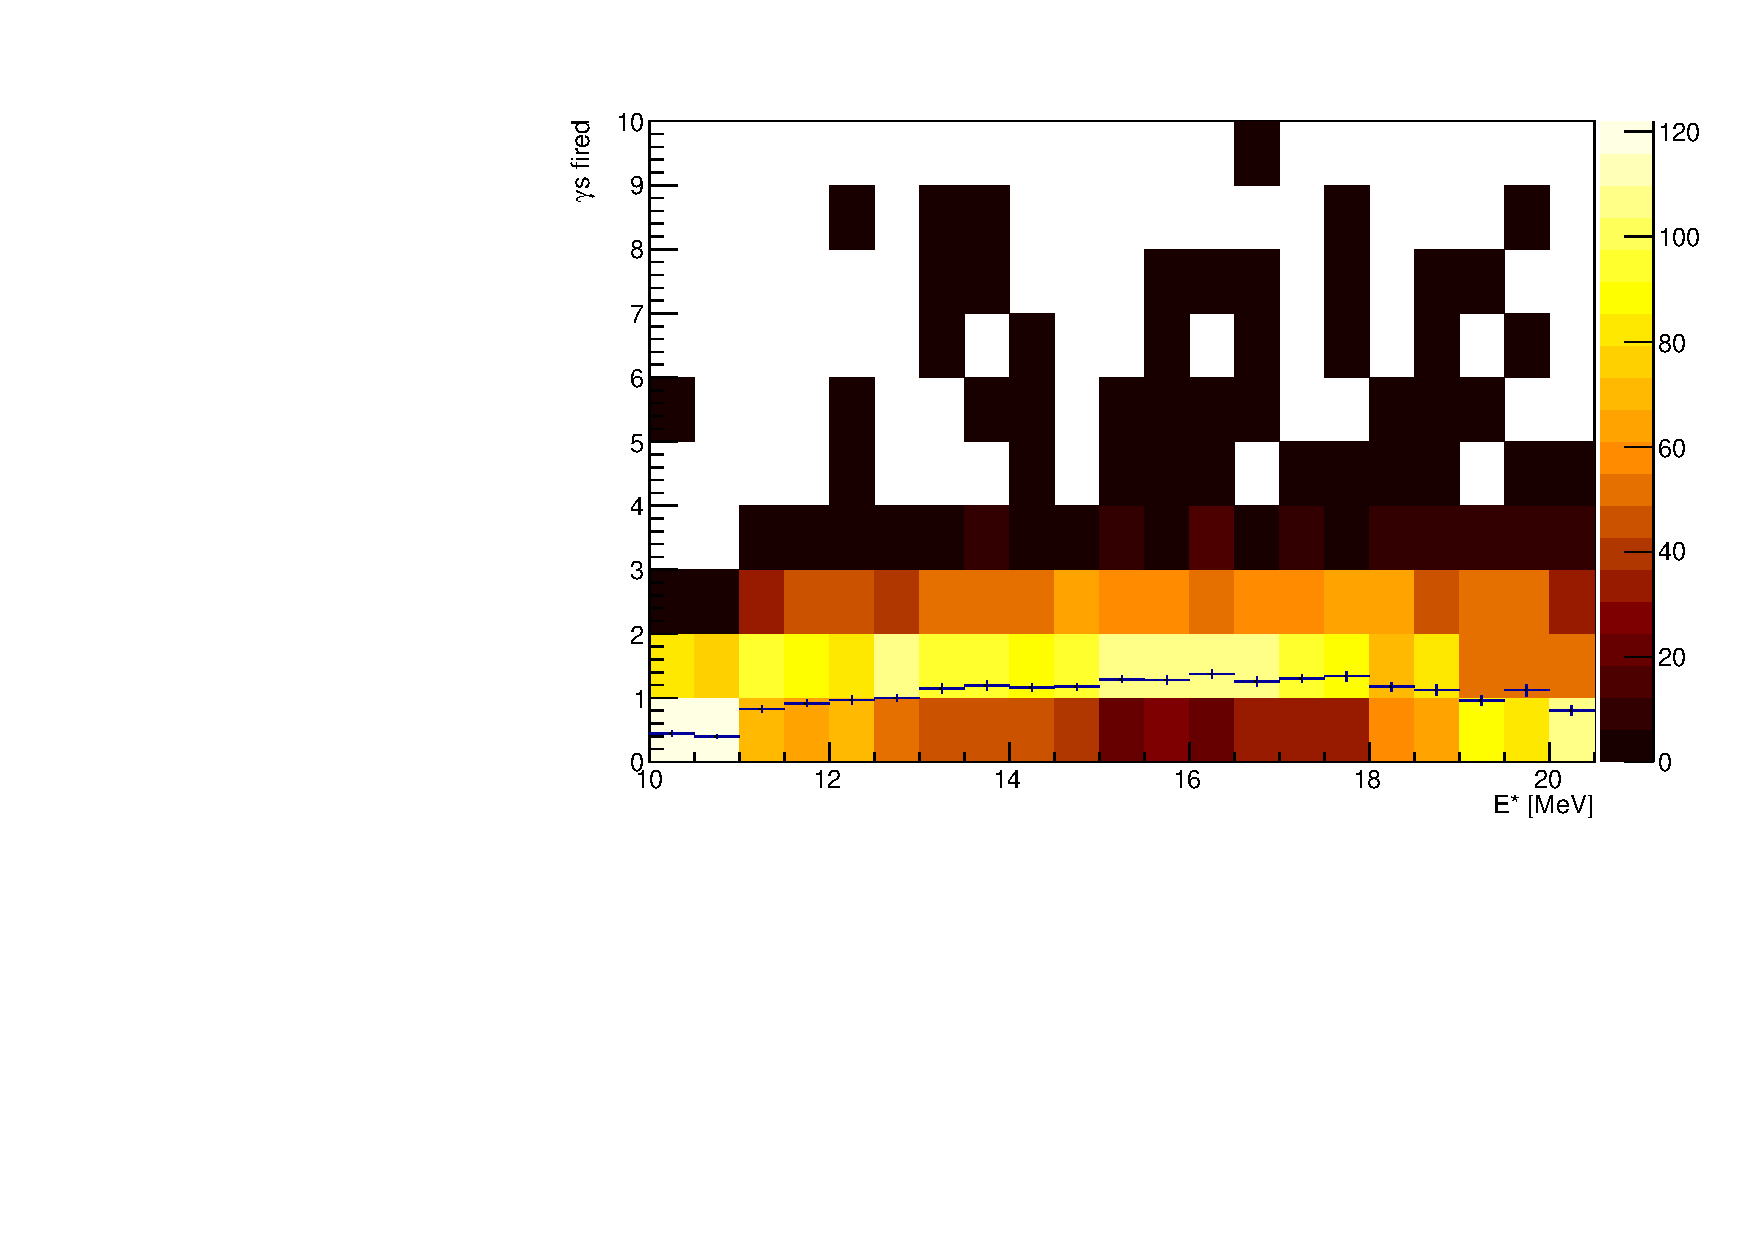
\includegraphics[width=\bredd\textwidth]{figures/gamma-mult/Ex-fg.pdf}}
\end{tabular}
\caption{\label{fig:gamma2} The gamma-multiplicities from simulations with $~^{17}\mathrm{N}$ at a kinetic energy $T=\unit[7123]{MeV}$ undergoing a quasi-elastic $(p,2p)$ reaction with a proton at rest in the origin. The simulations were performed for prefragment excitation energies $E*$ in the interval $[10,20]\,\unit{MeV}$ with a $\unit[0.5]{MeV}$ spacing.}
\end{center}
\end{figure}




%In \autoref{fig:XbEx}, we see the total energy deposited in the Crystal Ball, given as histograms for a different excitation energies. These are the energy deposits as given by the simulation: no addback routine has been run on them.
%Again, we see no obvious dependence: the average energy deposited is about $\unit[270]{MeV}$ for all excitation energies. This is perhaps not surprising given the narrow range of excitation energies, in comparison to the total energy deposited in the event. 
%\begin{figure}
%\begin{center}
%\includegraphics{figures/gamma-mult/Eex-XbsumE.pdf}
%\caption{\label{fig:XbEx} The total energy deposited in the Crystal Ball, for different excitation energies of the prefragment.}
%\end{center}
%\end{figure}

%Related to the